\documentclass[]{final_report}
\usepackage{graphicx}
\usepackage{hyperref}
\usepackage[normalem]{ulem}
\usepackage{amsmath}
\usepackage{csvsimple}
\usepackage{float}
\usepackage[]{algorithm2e}
\usepackage[noend]{algpseudocode}
\usepackage{url}
\usepackage{listings}             % Include the listings-package
\usepackage{enumerate}
\usepackage{cite}



\RestyleAlgo{boxruled}
\lstset{language=Python}
\newcommand{\myparagraph}[1]{\paragraph{#1}\mbox{}\\}

%%%%%%%%%%%%%%%%%%%%%%
%%% Project details
%%%%%%%%%%%%%%%%%%%%%%
\def\studentname{Kamil Smuga}
\def\projecttitle{An approach for Continuous Capacity Planning in Cloud Environments with an Uptime-based Pricing Model}
\def\supervisorname{Prof. Liam Murphy}
\def\moderatorname{Christina Thorpe}

\begin{document}

\maketitle
\tableofcontents\pdfbookmark[0]{Table of Contents}{toc}\newpage
\listoffigures\newpage
\par{\textbf{List of tables}}

%%%%
%The most important parts of your thesis are: abstract, introduction, conclusion and
%references. These are what get read first and make that vital initial impression.
%%%
%%%
%One of first things your examiners will look at is your literature review. If they see a
%good number of journal thesiss, a swathe of conference thesiss, a few recent workshop
%thesiss and not too many web sites, they’ll already be impressed.
%%%
%%%%%%%%%%%%%%%%%%%%%%
%%% ABSTRACT 
%%%%%%%%%%%%%%%%%%%%%%

\begin{abstract}

\textsl{New Infrastructure as a Service solutions are becoming available with a growing number of supported pricing models. A hosted Cloud environment can be a choice to design and build an infrastructure for a product. The recent availability of different pricing schemes based on resource utilization and uptime reveals new challenges in an already complex capacity planning process. There is a choice between ad-hoc provisioning and time commitment that comes with reduced hourly rates. When one decides for a time commitment, there are still further pricing options available. Few different prices for the same resource that depend on a daily uptime. Which one is the best one? When exactly does one pricing scheme becomes more cost effective that the other? We attempted to answer these critical questions by i) aggregating and transforming metrics data, ii) designing key optimality indicators, iii) using the indicators to build algorithms that suggest better configuration options, iv) using an existing large dataset to evaluate the algorithms. }

\end{abstract}
\newpage


Thanks to my wife Karen for her constant support and patience during the research and writing
of this Thesis.
Also, thanks to Prof. John Murphy and Viliam Holub for their support, help and assistance.

%%%%%%%%%%%%%%%%%%%%%%
%%% INTRODUCTION 
%%%%%%%%%%%%%%%%%%%%%%

\chapter{Introduction}

%%        *Some discussion to provide context

In recent years, Cloud Computing receives significant attention~\cite{6185529}~\cite{5741288}~\cite{5704303} and delivers infrastructure, platform and/or software as services over the Internet~\cite{7073248}. The popularity of cloud service encouraged many cloud service providers, like Amazon, Google, Microsoft, IBM and VMWare to come up with a range of provisioning and pricing schemes. The popular pay-as-you-go pricing model changes the usage patterns and influences the way capacity planning is done~\cite{6274129}. For example, one virtual machine configuration can have few different prices based on its uptime and pricing scheme. The dependency on uptime value is the central point of consideration in this thesis. We look from the perspective of Software as a Service (SaaS) provider that uses an Infrastructure as a Service (IaaS) provider's services to host a product. In this context, pricing and capacity planning are two important constituents of SaaS provider's success~\cite{6963393}.

%%        *A description of the problem

IaaS consumer can face a situation when resource-based capacity is known and it is time to rent an optimal machine configuration from the provider. It raises few open ended questions, including i) how many VMs is needed? ii) what kind of VMs and which pricing scheme? iii) how long should each VM run? In this thesis, we attempt to answer these questions in a cost-aware fashion considering uptime-based pricing models. It is a new consideration that adds uptime parameter to the standard resource-aware provisioning techniques~\cite{Bartolini:2014:AFC:2658949.2637480}.

%%        *Motivation for solving the problem

Answers to above questions have influence in two main cases 1) to decide on pricing of a product, 2) to optimize an existing configuration and bring savings.  The former is crucial for SaaS providers as they derive profits from the margin between the operational costs of infrastructure and revenue generated from customers~\cite{efficient_resource_allocation}. In other words, having this set right gives a competitive advantage and greatly contributes to a healthy business. The latter proved to yield savings up to 9.45\% that can be invested in other aspects of a business.   

%%        *A statement of the objectives

Motivated by a possibility to influence above factors, we propose a data-driven approach to solving this problem. Our objectives include:
\begin{enumerate}
\item Selection, collection and post-processing of crucial metrics that contribute to a final price and Service Level Agreements (SLAs).
\item Design and calculation of key indicators related to: i) total cost per hour (\textit{cph}), ii) exact points when one scheme becomes more optimal than the other - called intersection points (\textit{ip(scheme1, scheme2)}), iii) distance from intersection points (\textit{KDI}) used as a key indicator to categorize a single VM usage pattern.
\item Design and evaluation of two suggestion algorithms that take above data as an input and returns a new configuration suggestion and associated total cost.
\end{enumerate}

%%        *Related work (mention how your work is different/better)

Most of the related work is conducted from an IaaS provider perspective~\cite{6274129}~\cite{6253563} or aimed to find an optimal pricing state for providers and consumers to collaborate~\cite{6676685}~\cite{6963393}. This thesis is different in a way that it analyses a SaaS provider capacity planning in an environment when one resource have different prices tightly coupled with an uptime.

%%        *Describe the proposed solution

Our proposed solution implements listed objectives using mainly map-reduce jobs executed on Apache Spark\footnote{\url{https://spark.apache.org}} platform. Aggregations, key indicators and algorithms were designed, implemented in pseudo-code and Python and evaluated on Google cluster-usage trace~\cite{clusterdata:Reiss2011}. 

%%        *Mention some of the challenges

Main challenges include dealing with dynamic changes of pricing schemes offered by IaaS providers. Even though this thesis uses Amazon's related taxonomy, it should be read as an attempt to solve a general case for uptime-based variable pricing capacity planning. Other challenging aspect is a cost of migration to suggested environment. It was not considered in the results, however, it created an opportunity for future work to investigate an impact of the delta difference between an old and new configuration cost. Lastly, we hit a technical issues related to implementation and execution of aggregations and algorithms on large data sets. Jobs were failing due to not enough RAM capacity on a single machine. The issues were resolved by a combination of code improvements, like changing the way aggregations build hash-maps and an increase of parallelism and chunking granularity on the platform.

%%        *Describe the methodology (modelling and experimentation) and key overall result (e.g., Results show proposed approach can achieve a significant reduction in the cost by enabling a more optimal selection of VM types based on resource utilisation)

We used modelling and experimentation methodology to build and evaluate results. The SaaS provider perspective got represented by an availability of per task and per machine metrics. We came up with aggregations and key indicators that helped to characterise an existing state of the configuration. Then, we experimented with algorithms to design ones that can yield positive improvements in the total cost.
Results show proposed approach can achieve a meaningful reduction in the cost by enabling a more optimal assignment of VMs based on uptime and resource utilization. 

\myparagraph{Structure of the Thesis}\\
\textbf{Background}. This section outlines the background information related to IaaS consumer point of view and challenges related to finding the best configuration for the money. \par
\textbf{Design and Implementation}. This section explains design and environmental conditions for the aggregations, key indicators and algorithms. It also dives into implementation details on the Apache Spark platform. \par
\textbf{Evaluation}. The proposed map-reduce jobs and algorithms are evaluated on Google cluster-usage trace data. \par
\textbf{Conclusion and Future Work}. The suggestion results data and future work related to algorithm improvements are presented. 
 
\newpage

%%%%%%%%%%%%%%%%%%%%%%
%%% BACKGROUND 
%%%%%%%%%%%%%%%%%%%%%%

\chapter{Background}

\section{The Problem Domain} 

We look from the perspective of Software as a Service (SaaS) provider that uses an Infrastructure as a Service (IaaS) provider's services to host a product. \\
SaaS provider seeks i) predictable cost estimates and ii) the best value for money. The latter for obvious reasons - every healthy business is interested in minimizing the costs. The former is needed to set a right product pricing. Not too expensive and not too cheap. Failure to do so may ruin a business's budget. \\
IaaS provider pricing can be flexible as described in below sections. One instance configuration can have many prices based on a daily uptime. SaaS provider faces the challenge to pick the best one.



\section{Amazon EC2 pricing schemes}

A price of an instance in Amazon EC2 depends on its resources and pricing scheme it belongs to. As a result of the latter, one resource configuration can have few different prices. Amazon offers on-demand, spot and reserved instances billed hourly.

\paragraph{On-demand instances.} Allow to pay by the hour with no other commitments. The most expensive option.
\paragraph{Spot instances.} A real-time bidding platform. A customer can bid on price. Instance can run only when the bid exceeds current Spot Price.
\paragraph{Reserved instances.} Discounted price in comparison to On-demand in exchange of 1 or 3 years commitment. Guaranteed availability of reserved capacity. 

This thesis focuses around the concept of Reserved Instances. The scheme is further split into Light, Medium and Heavy options. They differ in upfront and hourly costs. Based on pricing data, Light serves well for short periods of daily usage, Heavy is optimized for long workloads and Medium is in between. \\
This scheme got simplified on December 2014~\cite{AWS:pricing_change} and naming used in this thesis does not match the latest offering anymore. However, the idea of having the same instance configuration priced differently based on uptime is still valid and is used by other IaaS providers, e.g. Google Compute Engine.

\section{Google Compute Engine pricing}

Google had greatly simplified the Compute Engine pricing. There is no concept of reservation nor bidding. All of the options are priced within pay-as-you-go model with 1 minute granularity. However, Google offers increasing discounts for sustained usage - 20\% for 25-50\% of month usage, 50-75\% of usage yields 40\% and everything above 75\% is priced with 60\% of discount rate. This is similar to the concept of Reserved Instances in a sense that uptime value influences a final price for the instance.

\section{Literature review}

Work related to IaaS market is focused either on provider's perspective~\cite{6274129}~\cite{6253563}, provider-consumer business interactions~\cite{6676685}~\cite{6963393} or consumer point of view~\cite{5961733}~\cite{6295066}. 

Authors of the paper~\cite{6253563} proposed a pricing framework for cloud services using game theory and data mining techniques. The framework determines the price based on recent usage data and available resources. It also takes into consideration various economic models and attempts to find the best price for provider and consumer at the same time.

In this paper~\cite{6274129}, authors focused on an analysis of pay-as-you-go flexible charging impact on IaaS provider's capacity planning. Their contribution was focused on cloud capacity estimation and management. Specifically, they developed a method to predict provisioning demand based on selected time series metrics. 
Although prediction is not included in this thesis, it would be a next logical step for future work to better address real-life use cases. 

IaaS consumer's optimal decisions were studied in the monopoly and multiple IaaS providers market~\cite{6963393}. Based on rational customer decisions, authors derived an optimal solution to provider's pricing problem. Furthermore, they modeled the pricing and capacity planning competition among the IaaS providers as a three-stage Stackelberg game and studied existence and conditions to achieve the Nash equilibrium. 

In the work conducted in paper~\cite{6676685}, authors proposed a two-stage provisioning scheme. At the first stage, they proposed a solution that works with flat and on-demand instances. Secondly, they studied bidding for the spot instances as a Stackelberg game. Although not focused on reserved instances, authors developed the system model that might serve as an inspiration for future work to provide suggestions based on application specific QoS metrics. 

Paper~\cite{5961733} described a cost-aware system that computed both a cost optimized configuration for the desired capacity as well as plan to migrate current setup to the proposed one. The cost-aware provisioning decisions are based on resource utilization and focused on finding the best resource configuration. Transition cost-aware provisioning included costs of migration and studied options to minimize it. 

A new algorithm was proposed to generate a resource provisioning scheme which minimizes the cost for customers and satisfies the application needs using branch and bound method~\cite{6295066}. Their main focus is to avoid over-provisioning and find the best resource configuration for given requirements. This thesis assumes that this work is already done and SaaS provider looks for the best pricing scheme configuration for an already known resource configuration.

%%%%%%%%%%%%%%%%%%%%%%
%%% DESIGN 
%%%%%%%%%%%%%%%%%%%%%%

\chapter{Design and Implementation}

\section{Taxonomy}
This section explains a terminology being used for further design and evaluation stages. It is important to re-define some terms, like cost per hour, which is sometimes presented by IaaS providers in a non-complete way and may not include all costs. We also define new terminology that will be used throughout this thesis.

\subsection{Upfront cost}

Investment in compute resources comes with an upfront cost. In case of a physical machines, it is hardware or lease cost. For virtual resources, a client can use IaaS provider services. These usually come with some fixed upfront cost and further per hour charges. \par

The upfront cost is considered to be a one-time payment and will be represented by \textit{u}.

\subsection{Cost per hour}

IaaS providers usually charge an X amount per hour. The charge might vary based on monthly uptime utilization or assigned pricing scheme. This number will be considered as a partial cost per hour and defined as \textit{pcph}. \\
Cost per hour represents a \textit{total cost} of running a single machine divided by number of hours in a calendar year. It includes upfront cost and per hour charges. It is defined as \textit{cph} and is a function of uptime hours per day summarized by equation~\ref{eq:cph}

\begin{equation}
\label{eq:cph}
cph(h) = \frac{u + \sum_{i=1}^{366} pcph \times h}{365 \times h}
\end{equation}

\subsection{Intersection points between pricing schemes}

Cost per hour is calculated for each of available pricing schemes. The single result represents a matrix of hours per day and \textit{cph}. Graphical representation of results produces a graph similar to Figure~\ref{fig:cc2_8xlarge}. \par 
\begin{figure}[H]
	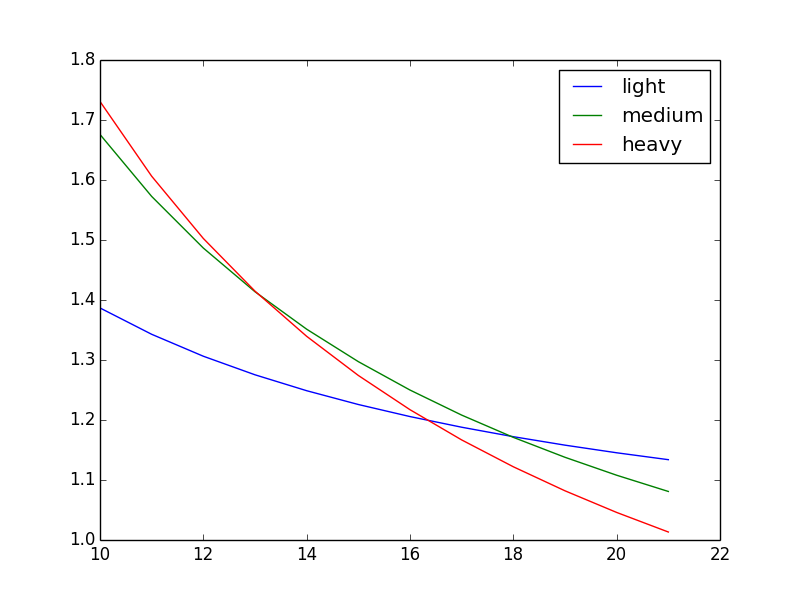
\includegraphics[width=\linewidth]{figures/cph_cc2_8xlarge_zoom}
	\caption{Zoomed \textit{cph} results for Amazon AWS cc2.8xlarge reserved instance rented for 1 year~\cite{AWS:light}~\cite{AWS:medium}~\cite{AWS:heavy}}
	\label{fig:cph_cc2_8xlarge_zoom}
\end{figure}

On the graph, there are visible intersections between pricing scheme's~\textit{cph}s. These points are an area of interest as they indicate when one scheme becomes more expensive than the other. For example, a light is the cheapest option to run for the first 16 hours a day. After this point, it is better to run a heavy utilization scheme. However, if we were to choose between medium and heavy, it would be better to run a medium for the first 13 hours. And between a medium and light, it makes sense to utilize light scheme for the first 18 hours and then switch to medium. 

\section{Algorithm}

The section contains design and implementation details for an end-to-end approach that analyzes machine configuration and proposes changes.
We start with metrics data prerequisites and guide through data transformations. We further define key indicators and formalize their implementations. The indicators can be used to filter non-optimal configurations. Algorithms that take the filter data as an input and generate configuration suggestions are presented later.

\subsection{Prerequisites} 

In order to make data-driven analysis and suggestions for optimization, we need data. We compiled a list of metrics that will be used as a source of truth to determine configuration's state. The list is suitable to measure performance SLAs for compute nodes. Machines with significant I/O usage profile are not covered in this thesis. 
Metrics can be gathered periodically, per process or per job. There are open source tools available to gather this data, e.g. collectd\footnote{\url{https://collectd.org}}, munin\footnote{\url{http://munin-monitoring.org}}, Logstash\footnote{\url{http://logstash.net}}.

The following list of metrics is required.
\myparagraph{Machine Id}
A unique machine ID. Used as a key to compute further analytics.

\myparagraph{Start and End Time}
Timestamps to indicate start and end of a measurement period.

\myparagraph{CPU usage}
Sampled or averaged CPU usage during a measurement period. 

\myparagraph{RAM usage}
Canonical memory usage measurement. 

Metrics should be aggregated in \textless K, List\textless V\textgreater\textgreater format where K represents Machine Id and List of V is a list of measurements in a given period. 

\subsection{Metrics data transformations and analytics}

Metrics gathered in Prerequisites section have limited knowledge about the environment. Collection per job or per process produces one log line and has a scope of a measurement period. Such structured data would not help to answer machine-wide nor cluster-wide questions. The data has to be post-processed to allow calculation of below-listed aggregations and analytics.   

\myparagraph{Daily usage}

To comply with IaaS pricing strategies, the data is analyzed in terms of a daily usage. This requires splitting metrics into buckets of one day worth of data. 
It is achieved by applying a simple Apache Spark filter presented in Listing~\ref{daily_usage} that calculates an integer to indicate a day number based on a metric timestamp. The implementation can vary for various timestamp formats. Results can be saved in separated folders or tables and all other aggregations and transformations are executed in scope of 1 day worth of data.

\begin{minipage}{\textwidth}
\begin{lstlisting}[label={daily_usage},caption={Daily usage filter},frame=single]

def daily_filter(line):
    day_data = line.split(",")[1]
    if (day_data == day):
        return True
    else:
        return False

for x in range(0, days_range):
    split_by_day = distFile.filter(daily_filter)

\end{lstlisting} 
\end{minipage}


\myparagraph{Uptime per machine}

This metric indicates a daily number of hours of machine being up. It is a key metric that is be used to calculate optimality indicators discussed in the next three following paragraphs. Algorithm~\ref{alg:uptime_per_machine} represents pseudo-code implementation and Listing~\ref{uptime_per_machine_implementation} contains implementation in Python with Apache Spark. The data is extracted from timestamp values previously grouped into daily data buckets. By design, this approach extracts start and end time of jobs recorded in metrics using map function (lines 1-2). Then, two reduce jobs are executed that find the earliest start time (lines 3-4) and the latest end time (lines 5-6). As a result, we get two timestamps that indicate a range of a daily uptime. This design is flawed in a sense that if there are only two jobs logged - one in the morning and one in the evening - it will assume that machine was up no matter what happened in between.

\begin{algorithm}[h]
\caption{Uptime per machine}
\label{alg:uptime_per_machine}
 \KwData{Task start and end time in a form of \textless K, List\textless V\textgreater\textgreater where K is Machine ID}
 \KwResult{Number of uptime hours per machine per day}
 \algrenewcommand\algorithmicfunction{\textbf{class}}
 \algrenewcommand\algorithmicprocedure{\textbf{method}}
  \begin{algorithmic}[1]
        \Procedure{map}{$\textrm{Id } key, \textrm{List } values}$
                \State $\textsc{Emit}(\textrm{Id }key, (startTime, endTime))$
        \EndProcedure
        \Procedure{reduce for min start time}{$\textrm{Id } key, \textrm{Tuple } values}$
                \State $\textsc{Emit}(\textrm{Id }key, (a < b) ? a : b)$
        \EndProcedure
        \Procedure{reduce for max end time}{$\textrm{Id } key, \textrm{Tuple } values}$
                \State $\textsc{Emit}(\textrm{Id }key, (a > b) ? a : b)$
        \EndProcedure
  \end{algorithmic}
\end{algorithm}

\begin{minipage}{\linewidth}
\begin{lstlisting}[label={uptime_per_machine_implementation},caption={Uptime per machine implementation in Apache Spark},frame=single] 
min_start = distFile.map(lambda(line): 
                (line.split(",")[0], line.split(",")[2]))
                .reduceByKey(lambda a,b: a if a<b else b)

max_end = distFile.map(lambda(line): 
                (line.split(",")[0], line.split(",")[3]))
                .reduceByKey(lambda a,b: a if a>b else b)
\end{lstlisting}
\end{minipage}

\myparagraph{Cost per hour}

This is an implementation of \textit{cph} metric~\ref{eq:cph} defined in Taxonomy. Algorithm~\ref{alg:cost_per_hour} represents pseudo-code and Listing~\ref{cost_per_hour} shows implementation in Python. 
The algorithm takes upfront cost, charge per hour and daily uptime as input parameters. It aggregates both costs and calculates a real (total) cost per hour~\textit{if} machine were to run every day for a number of previously specified hours. We use this algorithm to build lookup tables for a 24 hour usage period. Essentially, we pass the same pricing scheme parameters and specify daily uptime from 1 to 24. This creates a table with hours per day to~\textit{cph} mapping.

\begin{algorithm}[H]
 \caption{Cost per hour}
 \label{alg:cost_per_hour}
 \KwData{Upfront cost, Charge per hour, Uptime [hours per day];}
 \KwResult{Total cost per hour for a given pricing scheme defined as \textit{cph};}
 return (upfront + (365 * perhour * hours)) / (365 * hours)
\end{algorithm}

\begin{minipage}{\linewidth}
\begin{lstlisting}[label={cost_per_hour},caption={Cost per hour implementation in Python},frame=single] 
def _calc_cost_per_hour(self, upfront, cost_per_hour, hours_per_day):
        return (upfront + (365 * cost_per_hour * hours_per_day)) /
                (365 * hours_per_day)
\end{lstlisting}
\end{minipage}

\myparagraph{Intersection points}

This is an implementation of \textit{ip(scheme1, scheme2)} metric defined in Taxonomy. This represents a reference point that finds intersections of~\textit{cph}s for various schemes. Algorithm~\ref{alg:intersection points} represents pseudo-code and Listing~\ref{intersection_points} shows implementation in Python. 

\begin{algorithm}[H]
 \label{alg:intersection points}
 \KwData{Array of cph for 2 pricing schemes;}
 \KwResult{Intersection point when one pricing scheme becomes cheaper than the other one;}
 read array1\;
 read array2\;
 \ForAll{cph in array} {
 	\If{$cph2 <= $cph1} {
 		return cph
 	}
 }
\caption{Calculate intersection point between two pricing schemes}
\end{algorithm}

\begin{minipage}{\linewidth}
\begin{lstlisting}[label={intersection_points},caption={Intersection point between various pricing schemes},frame=single] 
def _calc_intersection_point(self, first, second):
   for i in range(len(first)):
      if (second[i] <= first[i]):
         return i
\end{lstlisting}
\end{minipage}

\myparagraph{Key Distance Indicator}

This metric represents a distance from intersection points calculated based on uptime. The result can be negative - to indicate a non-optimal profile - or positive otherwise. Positive and negative values can be yielded in either direction of the time axis as presented in Figure~\ref{fig:distance}. 

\begin{figure}[H]
       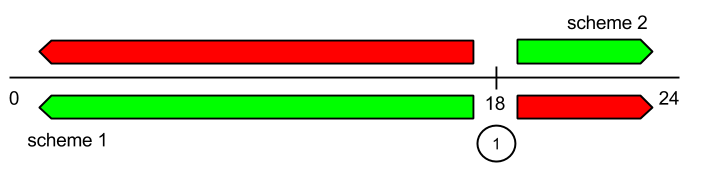
\includegraphics[width=\linewidth]{figures/distance}
      \caption{Distance from intersection points. Positive (green) values indicate the optimal result. Negative (red) represent data for further improvement.}
        \label{fig:distance}
\end{figure}

At 18 hours, the point of scheme cost intersection (highlighted as 1), it does not matter which scheme is chosen as cost is the same. This is point 0.
At each side of the intersection point either scheme1 or scheme 2 is more preferable.
For example, a machine running for 20 hours on scheme1 is running 2 hours outside our optimum 18 hour scheme cost intersection. This gives us a score of -2 for this machine compared to the same machine running on scheme 2 where the benefits continue to increase the longer the machine is running.
The same is true for a machine running for 10 hours on scheme 2. We are running at -8 below our optimum. In this case we would be more cost beneficial to run this machine on scheme1. Giving us a score of +8.

Algorithm~\ref{alg:distance_from_optimality} represents pseudo-code implementation.


\begin{algorithm}[H]
 \label{alg:distance_from_optimality}
 \KwData{Uptime, Intersection Point, Bias;}
 \KwResult{Distance from intersection point [-24, 24];}
  \If{Bias} {
        return Uptime - Intersection Point
  } 
  \Else{
        return Intersection Point - Uptime
  }
\caption{Uptime Based Distance From Intersection Points}
\end{algorithm}

\subsection{Recognition of inefficiencies and suggestions for changes}

\myparagraph{Threshold Based Report}

A user can define which KDI value is non-optimal and run a report to find machines below this point. For example, every negative KDI value signalizes there is a better pricing scheme available. A user can catch this situation by having a threshold value set to 0. However, there might be a situation when machine is taken for maintenance and reports negative values for one or a couple of days. To avoid this kind of noise, a user can add an another criteria to specify a minimum number of days of reported values below the threshold.

\myparagraph{Aggregated CPU and memory usage}

An aggregated daily values of CPU and memory will help to suggest better utilization strategies that guarantee SLAs. Algorithm~\ref{alg:agg_cpu_mem} represents pseudo-code implementation and~\ref{agg_cpu_mem_implementation} contains implementation in Python with Apache Spark. The algorithm takes metrics data grouped by keys that represent machine IDs and list of values as an input. It extracts CPU and memory usage using map function (lines 1-2). Then, uses the same reduce function to calculate a sum for each of the metrics (lines 3-4) per machine.

\begin{algorithm}[h]
\caption{Aggregated CPU and memory}
\label{alg:agg_cpu_mem}
 \KwData{CPU and memory usage in a form of \textless K, List\textless V\textgreater\textgreater where K is Machine ID}
 \KwResult{Aggregated CPU and memory usage}
 \algrenewcommand\algorithmicfunction{\textbf{class}}
 \algrenewcommand\algorithmicprocedure{\textbf{method}}
  \begin{algorithmic}[1]
        \Procedure{map}{$\textrm{Id } key, \textrm{List } values}$
                \State $\textsc{Emit}(\textrm{Id }key, (cpuUsage, memoryUsage))$
        \EndProcedure
        \Procedure{reduce}{$\textrm{Id } key, \textrm{Int } aggValue}$
                \State $\textsc{Emit}(\textrm{Id }key, a + b)$
        \EndProcedure
  \end{algorithmic}
\end{algorithm}

\begin{minipage}{\linewidth}
\begin{lstlisting}[label={agg_cpu_mem_implementation},caption={Aggregated CPU and memory implementation in Apache Spark},frame=single] 
cpu = distFile.map(lambda(line): 
                (line.split(",")[0], line.split(",")[5]))
            .reduceByKey(lambda a,b: a + b)

mem = distFile.map(lambda(line): 
                (line.split(",")[0], line.split(",")[6]))
            .reduceByKey(lambda a,b: a + b)
\end{lstlisting}
\end{minipage}

\myparagraph{Calculate number of jobs per day}

The number of jobs per day is a useful parameter to calculate cluster-wide averages used for suggestions. Algorithm~\ref{alg:jobs_per_day} represents pseudo-code implementation and~\ref{jobs_per_day} contains implementation in Python with Apache Spark. Similarly to the previous algorithms, this one takes metrics data grouped by keys that represent machine IDs and list of values as an input. It extracts a task usage information using map function (lines 1-2). Then, it uses a reduce function to calculate an aggregated cluster value (lines 3-4) per machine.

\begin{algorithm}[h]
\caption{Daily jobs count}
\label{alg:jobs_per_day}
 \KwData{Job entry in a form of \textless K, List\textless V\textgreater\textgreater where K is Machine ID}
 \KwResult{Aggregated jobs count}
 \algrenewcommand\algorithmicfunction{\textbf{class}}
 \algrenewcommand\algorithmicprocedure{\textbf{method}}
  \begin{algorithmic}[1]
        \Procedure{map}{$\textrm{Id } key, \textrm{List } values}$
                \State $\textsc{Emit}(\textrm{Id }key, 1)$
        \EndProcedure
        \Procedure{reduce}{$\textrm{Id } key, \textrm{Int } aggValue}$
                \State $\textsc{Emit}(\textrm{Id }key, a + b)$
        \EndProcedure
  \end{algorithmic}
\end{algorithm}

\begin{minipage}{\linewidth}
\begin{lstlisting}[label={jobs_per_day},caption={Aggregated CPU and memory implementation in Apache Spark},frame=single] 
def mapping(line):
    machine_id = line.split(",")[0]
    counter = 1
    return (machine_id, counter)

task_counter = distFile.map(mapping).reduceByKey(add)
\end{lstlisting}
\end{minipage}


\subsubsection{Squeeze-them-in suggestion strategy}

The proposed strategy calculates an amount of spare CPU and memory capacity based on cluster-wide averages. An aggregated value for CPU and memory represents an amount of capacity gathered from machines that are utilized below the average. Based on the amount of an aggregated capacity, the algorithm attempts to squeeze in a maximum amount of machines returned by a threshold-based report. As a result, it proposes to turn off some number of machines that can fit in the previously calculated below-average capacity. \\
This approach has a potential to perform well in under-utilized clusters. For well-balanced environments with similar usage patterns, it does not find a lot of spare capacity and would propose fairly limited improvements. \\
A pseudo-code implementation of this idea is presented in Algorithm~\ref{alg:squeeze-them-in}.

\begin{algorithm}[h]
\caption{Squeeze them in suggestion strategy}
\label{alg:squeeze-them-in}
 \KwData{Cluster averages for CPU and memory, List of machines from Threshold Based Report, List of other machines}
 \KwResult{List of machines that can be powered down}
 \algrenewcommand\algorithmicfunction{\textbf{class}}
 \algrenewcommand\algorithmicprocedure{\textbf{method}}
 \begin{algorithmic}[1]
  $float spareCpu = 0;$
  $float spareMemory = 0;$
  $ID[ ] machinesToExclude;$

\ForAll{machine in otherMachines}{
        \If{$machine.cpu < cluster.cpu$} {
                 $spareCpu += clusterCpu - machineCpu$
        }
        \If{$machine.memory < cluster.memory$} {
        	$spareMemory += clusterMemory - machineMemory$
        }
}

\ForAll{machine in machinesFromReport}{
        \If{$(spareCpu - machine.cpu > 0) \&\& (spareMemory - machine.memory > 0)$}{
                add machine to machinesToExclude;
        }
}

\Return machinesToExclude;
\end{algorithmic}
\end{algorithm}

\subsubsection{New capacity configuration suggestion}

New configuration is calculated based on input from the report, list of available schemes and total uptime to handle. Pseudo-code implementation is presented in Algorithm~\ref{alg:new_configuration}. The algorithm iterates through all of available schemes, reads \textit{intersection points} and gets \textit{cph} for each of the \textit{ip}s. It returns a total cost and number of machines required for each proposed configuration. \\
Suggestion results are limited to one type of pricing scheme. In reality, there might be a more optimal solution yielded from mixing pricing schemes. 

\begin{algorithm}[h]
\caption{New configuration suggestion}
\label{alg:new_configuration}
 \KwData{List of machines from Threshold Based Report, List of available schemes, Total uptime;}
 \KwResult{New configuration suggestion}
 \algrenewcommand\algorithmicfunction{\textbf{class}}
 \algrenewcommand\algorithmicprocedure{\textbf{method}}

  $float[ ] totalCost;$

\ForAll{scheme in availableSchemes}{
		\ForAll{ip in scheme.intersectionPoints}{
			vms = Uptime / ip.getHours() \\
			cost = ip.getCphForHours(ip.getHours()) \\
			totalCost[ip] = (vms, cost)
		}
}

\Return{totalCost}
\end{algorithm}



%%%%%%%%%%%%%%%%%%%%%%  
%%% EVALUATION!!!
%%% ALGORITHM TESTING  
%%% ON GOOGLE DATASET 
%%%%%%%%%%%%%%%%%%%%%%

\chapter{Evaluation}

\section{Methodology}

Evaluation process can be split into four phases:
\begin{enumerate}
\item collection and transformation of pricing and usage data,
\item calculation of key indicators (\textit{cph, ip(scheme1, scheme2), KDI}) and cluster characteristics (\textit{total cost, performance averages}), 
\item suggestion of changes based on Algorithm~\ref{alg:squeeze-them-in} and~\ref{alg:new_configuration},
\item validation of a positive correlation between \textit{KDI} and \textit{total cost} changes.
\end{enumerate}

\section{Setup description}

\myparagraph{Workstation}
Hardware - Intel Xeon 6-core x86\_64 2.4GHz, L3 cache 24MB, RAM 28GB. \\
Operating System - OS X Yosemite 10.10.2

\myparagraph{Platform}
Apache Spark 1.2.1\footnote{\url{https://spark.apache.org}} - an engine for large-scale data processing. All of the map-reduce jobs were written using Python API. Jobs were executed using standalone cluster mode with settings specified in Table~\ref{tab:spark_conf}. Job run times varied widely based on input data size and complexity of computations - from 20hs+ for transformations on 100G+ data to 1-minute aggregations on 100-200M input.

\begin{table}[h]
\begin{center}
    \begin{tabular}{| l | l |}
    \hline
    \textbf{Setting name} & \textbf{Value} \\
    \hline
    spark.master & local \\
    \hline
    spark.driver.memory & 8G \\
    \hline
    spark.executor.memory & 20G \\
    \hline
    spark.default.parallelism & 500 \\
    \hline
    \end{tabular}
\end{center}
\caption{Apache Spark standalone cluster configuration settings} 
\label{tab:spark_conf}
\end{table}

Settings were tweaked during computation mostly due to frequent Out Of Memory errors. Default driver and executor settings - 256M and 512M respectively - were not enough to handle the volume of input data. Further OOMs occurred during \textit{RRD.reduceByKey}\footnote{\url{https://spark.apache.org/docs/1.2.1/api/python/pyspark.html\#pyspark.RDD.reduceByKey}} operations as it required to compute a fairly large hash map. Tweaks of \textit{spark.default.parallelism} setting worked the best as it enforced more granular input data chunking.

\section{Input data}

\myparagraph{Pricing data}

Amazon Web Services\footnote{\url{http://aws.amazon.com/}} offered variable pricing schemes based on uptime. Customer could choose an instance configuration and total cost would be calculated based on a number of hours of uptime per day.
The offering was split into three options:
\begin{enumerate}
\item light - low upfront and high per hour cost,
\item medium - medium upfront and medium per hour cost,
\item heavy - high upfront and low per hour cost.
\end{enumerate}

For evaluation purposes, we choose two pricing schemes for two different VM configurations~\cite{AWS:light}~\cite{AWS:medium}~\cite{AWS:heavy}. Pricing details are specified in Table~\ref{tab:aws_pricing}

\begin{table}[h]
\begin{center}
    \begin{tabular}{| l | l | l | l |}
    \hline
    \textbf{Name} & \textbf{Scheme} & \textbf{Upfront (\$)} & \textbf{Per hour (\$)} \\
    \hline
    cc2.8xlarge & light & 1762 & 0.904 \\
    \hline
    cc2.8xlarge & medium & 4146 & 0.54 \\
    \hline
    cc2.8xlarge & heavy & 5000 & 0.361 \\
    \hline
    m2.4xlarge & light & 1088 & 0.676 \\
    \hline
    m2.4xlarge & medium & 2604 & 0.52 \\
    \hline
    m2.4xlarge & heavy & 3156 & 0.272 \\
    \hline
    \end{tabular}
\end{center}
\caption{AWS pricing for reserved cc2.8xlarge and m2.4xlarge instances}
\label{tab:aws_pricing}
\end{table}

\myparagraph{Usage data}

Google released 29-day cluster usage traces of more than 12k machines that run over 650k jobs~\cite{clusterdata:Reiss2011}. An analysis~\cite{clusterdata:Reiss2012b} revealed that the workload is heterogeneous, which is somewhat unique compared to other traces and makes a good fit for testing.
The trace contains data about jobs submitted by users. Each job is made of tasks. Each task reports metrics about resource consumption - e.g. CPU, memory - and timestamps. The trace does not contain information about the purpose of the jobs, which limits SLA assumptions to resource utilization. 
Resource utilization data is provided in normalized units - the strongest configuration is 1 and the rest of configurations are described in relation to that value.

\myparagraph{Pricing assignment to usage data}

Google trace does not provide any information about pricing schemes of included machines. For evaluation purposes, we will produce example configurations of different pricing schemes that could exist within a real cluster. 

The majority of machines within Google cluster i.e. 82\%, have following configuration: 0.5 CPU, 0.5 RAM or 0.5 CPU, 0.25 RAM. We will assign heavy pricing scheme for these machines. For the rest of the cluster, we will assign medium pricing scheme. 
As a result of the assignment cluster machines are grouped into 10595 machines of heavy and 2258 of medium usage.

The light scheme is a good fit for relatively short periods of time, e.g. during peak. An analysis of the trace~\cite{clusterdata:Reiss2012b} shows that jobs with the highest peak-to-mean ratio are production priority jobs and they constitute only 7\% of all jobs. Therefore, we will not assign any light pricing schemes for this evaluation purposes. 

We will refer to cc2.8xlarge and m2.4xlarge reserved instances pricing data as \textit{Scheme 1} and \textit{Scheme 2}.  
 

\section{Schema transformations and aggregations}

Google trace data contains a lot of detailed information. This thesis focuses on uptime and we extracted only relevant data for further evaluation. Machine and task events original schema is presented in Tables~\ref{tab:machine_events} and~\ref{tab:task_events} and fields selected for further transformation and aggregation are marked in bold text. 

\begin{table}[h]
\begin{center}
    \begin{tabular}{| l | l |}
    \hline
    & \textbf{Column name} \\
    \hline
    1 & \textbf{timestamp}\\
    \hline
    2 & \textbf{machine id} \\
     \hline
    3 & event type\\
     \hline
    4 & platform id\\
     \hline
    5 & \textbf{capacity: CPU}\\
     \hline
    6 & \textbf{capacity: memory}\\
    \hline
    \end{tabular}
\end{center}
\caption{Machine events table schema from Google trace}
\label{tab:machine_events}
\end{table}


\begin{table}[h]
\begin{center}
    \begin{tabular}{| l | l |}
    \hline
    & \textbf{Column name} \\
    \hline
    1 & \textbf{start time of the measurement period}\\
    \hline
    2 & \textbf{end time of the measurement period}\\
     \hline
    3 & job ID\\
     \hline
    4 & task index\\
     \hline
    5 & \textbf{machine ID} \\
     \hline
    6 & mean CPU usage rate \\
    \hline
    7 & \textbf{canonical memory usage}\\
    \hline
    8 & assigned memory usage\\
    \hline
    9 & unmapped page cache memory usage\\
    \hline
    10 & total page cache memory usage\\
    \hline
    11 & maximum memory usage\\
    \hline
    12 & mean disk I/O time\\
    \hline
    13 & mean local disk space used\\
    \hline
    14 & maximum CPU usage\\
    \hline
    15 & maximum disk IO time\\
    \hline
    16 & cycles per instruction (CPI)\\
    \hline
    17 & memory accesses per instruction\\
    \hline
    18 & sample portion\\
    \hline
    19 & aggregation type \\
    \hline    
    20 & \textbf{sampled CPU usage}\\
    \hline
    \end{tabular}
\end{center}
\caption{Task events table schema from Google trace}
\label{tab:task_events}
\end{table}

\begin{table}[h]
\begin{center}
    \begin{tabular}{| l | l |}
    \hline
    & \textbf{Column name} \\
    \hline
    1& machine ID\\
    \hline
    2 & total CPU usage\\
     \hline
    3 & CPU capacity\\
     \hline
    4 & total assigned memory usage\\
     \hline
    5 & memory capacity\\
     \hline
    6 & number of tasks\\
    \hline
    \end{tabular}
\end{center}
\caption{Aggregated statistics from Google trace data}
\label{tab:new_schema}
\end{table}

Table~\ref{tab:new_schema} is a new schema produced from join of capacity metrics from machine events and aggregations computed from tasks events data. 

\myparagraph{Daily usage}
As a first step, the task usage data is grouped into separate buckets to represent 1 day worth of data based on timestamps. Listing~\ref{daily_usage} shows Apache Spark filter implementation in Python. This transformation created 29 folders of data.

\myparagraph{Uptime}
Uptime per day per machine was calculated based on an aggregation of task duration times for a given day. Algorithm~\ref{alg:uptime_per_machine} shows design and Listing~\ref{uptime_per_machine_implementation} represents the implementation of this aggregation. The total number of hours in the cluster is 8705743, which gives 23.36 hours daily per machine on average. 

\myparagraph{Total CPU and memory usage}
CPU and memory aggregation logic is presented in Algorithm~\ref{alg:agg_cpu_mem} and implemented in Listing~\ref{agg_cpu_mem_implementation}. The total CPU consumption of the cluster is 15972217.38, which gives 43.77 daily per machine on average. The total memory usage is 30676363.36, which is 84.06 on average. 

\myparagraph{Total number of tasks}
An aggregated number of tasks is calculated based on Algorithm~\ref{alg:jobs_per_day} and implementation presented in Listing~\ref{jobs_per_day}. The total number of tasks is 1234716525, which gives 3383.65 tasks per day per machine on average.


\section{Pricing data indicators}

\subsection{Cost per hour}

Based on Formula~\ref{eq:cph} implemented in Python and presented in Listing~\ref{cost_per_hour}, we calculated a \textit{cost per hour} for both analyzed schemes. Results are presented in Table~\ref{tab:cph:scheme1} and~\ref{tab:cph:scheme2} in respect of number of hours per day a machine would run. The cost per hour drops when uptime per day rises. The same trend exhibits for both schemes.

\myparagraph{Scheme1}
\begin{table}[h]
\begin{center}
    \begin{tabular}{| l | l | l | l |}
    \hline
    \textbf{Hour} & \textbf{Light (price/hour)} & \textbf{Medium (price/hour)} & \textbf{Heavy (price/hour)} \\
    \hline
	1&5.7313972602739724&11.898904109589042&14.059630136986302 \\
    \hline
	2&3.317698630136986&6.2194520547945205&7.21031506849315 \\
    \hline
	3&2.513132420091324&4.326301369863014&4.9272100456621 \\
    \hline
	4&2.110849315068493&3.3797260273972602&3.785657534246575 \\    
	\hline
  5&1.8694794520547946&2.811780821917808&3.1007260273972603 \\
  	\hline
  6&1.7085662100456622&2.433150684931507&2.64410502283105 \\
  	\hline 
  7&1.593628180039139&2.162700587084149&2.317947162426614 \\
  \hline 
  8&1.5074246575342467&1.9598630136986301&2.0733287671232876 \\
  \hline
  9&1.4403774733637749&1.8021004566210044&1.8830700152207003 \\
  \hline
  10&1.3867397260273973&1.6758904109589041&1.73086301369863 \\ 
  \hline
  11&1.342854296388543&1.5726276463262765&1.6063300124533002 \\ 
  \hline
  12&1.3062831050228312&1.4865753424657535&1.5025525114155251 \\
  \hline
  13&1.2753382507903057&1.4137618545837725&1.414740779768177 \\
  \hline
  14&1.2488140900195697&1.3513502935420745&1.3394735812133072 \\
  \hline
  15&1.2258264840182649&1.2972602739726027&1.2742420091324203 \\
  \hline
  16&1.2057123287671234&1.249931506849315&1.2171643835616437 \\
  \hline
  17&1.1879645447219984&1.208170829975826&1.1668017727639 \\
  \hline
  18&1.1721887366818875&1.1710502283105022&1.12203500761035 \\ 
  \hline
  19&1.1580735400144198&1.1378370583994233&1.0819805335255948 \\
  \hline
  20&1.1453698630136988&1.107945205479452&1.045931506849315 \\
  \hline
  21&1.1338760600130462&1.0809001956947162&1.0133157208088714 \\
  \hline
  22&1.1234271481942715&1.0563138231631384&0.9836650062266501 \\
  \hline
  23&1.1138868374032165&1.0338653960690887&0.9565926146515782 \\ 
  \hline
  24&1.1051415525114157&1.0132876712328769&0.9317762557077626 \\ 
    \hline
    \end{tabular}
\end{center}
\caption{cph results for cc2.8xlarge reserved instance}
\label{tab:cph:scheme1}
\end{table}

\myparagraph{Scheme2}

\begin{table}[h]
\begin{center}
    \begin{tabular}{| l | l | l | l |}
    \hline
    \textbf{Hour} & \textbf{Light (price/hour)} & \textbf{Medium (price/hour)} & \textbf{Heavy (price/hour)} \\
    \hline
1&3.656821917808219&7.654246575342467&8.918575342465754\\ 
 \hline 
2&2.1664109589041094&4.087123287671233&4.595287671232876\\ 
 \hline 
3&1.669607305936073&2.898082191780822&3.1541917808219178\\ 
 \hline 
4&1.4212054794520548&2.303561643835616&2.4336438356164383\\ 
 \hline 
5&1.2721643835616436&1.9468493150684931&2.0013150684931507\\ 
 \hline 
6&1.1728036529680366&1.709041095890411&1.713095890410959\\ 
 \hline 
7&1.1018317025440314&1.5391780821917809&1.5072250489236791\\ 
 \hline 
8&1.0486027397260274&1.411780821917808&1.352821917808219\\ 
 \hline 
9&1.0072024353120244&1.3126940639269407&1.2327305936073059\\ 
 \hline 
10&0.9740821917808219&1.2334246575342467&1.1366575342465755\\ 
 \hline 
11&0.9469838107098382&1.1685678704856788&1.058052303860523\\ 
 \hline 
12&0.9244018264840183&1.1145205479452056&0.9925479452054796\\ 
 \hline 
13&0.9052939936775553&1.0687881981032665&0.9371211801896734\\ 
 \hline 
14&0.8889158512720158&1.0295890410958906&0.8896125244618396\\ 
 \hline 
15&0.8747214611872147&0.9956164383561644&0.8484383561643836\\ 
 \hline 
16&0.8623013698630138&0.9658904109589042&0.8124109589041095\\ 
 \hline 
17&0.8513424657534246&0.9396615632554393&0.7806220789685737\\ 
 \hline 
18&0.8416012176560121&0.9163470319634702&0.7523652968036529\\ 
 \hline 
19&0.8328853640951694&0.8954866618601299&0.7270829127613554\\ 
 \hline 
20&0.825041095890411&0.8767123287671232&0.7043287671232877\\ 
 \hline 
21&0.8179439008480104&0.8597260273972603&0.6837416829745597\\ 
 \hline 
22&0.8114919053549191&0.8442839352428394&0.6650261519302615\\ 
 \hline 
23&0.8056009529481835&0.8301846337105421&0.6479380583680763\\ 
 \hline 
24&0.8002009132420091&0.8172602739726028&0.6322739726027398 \\
 \hline 
    \end{tabular}
\end{center}
\caption{cph results for m2.4xlarge reserved instance}
\label{tab:cph:scheme2}
\end{table}

\subsection{Intersection points}

Based on Formula~\ref{alg:intersection points} implemented in Python and presented in Listing~\ref{intersection_points} we calculated \textit{intersection points} between pricing schemes. Table~\ref{tab:intersection_points} shows results of the calculation. Intuitively, a heavy scheme is the cheapest option for highly utilized machines. An interesting finding is that a medium is never cheaper than light in case of Scheme 2. Figures~\ref{fig:cc2_8xlarge} and~\ref{fig:m2_4xlarge} represent graphically \textit{cph} results and \textit{intersection points} can be noticed.

\begin{table}[h]
\begin{center}
    \begin{tabular}{| l | l | l |}
    \hline
    & \textbf{Scheme 1} & \textbf{Scheme 2} \\
    \hline
    light/medium & 17 & never \\
    \hline
    light/heavy & 16 & 6 \\
    \hline
    medium/heavy & 13 & 14 \\
    \hline
    \end{tabular}
\end{center}
\caption{Intersection points for Scheme 1 and Scheme 2}
\label{tab:intersection_points}
\end{table}

\begin{figure}[H]
  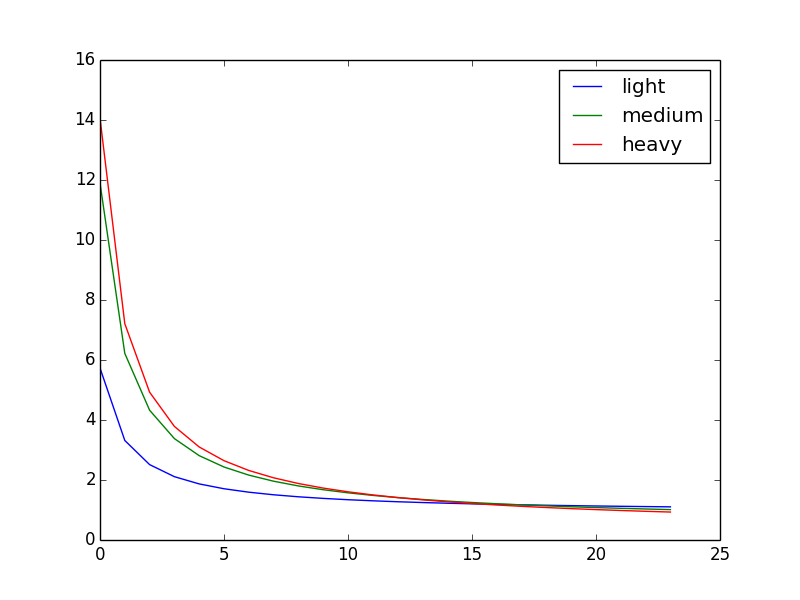
\includegraphics[width=\linewidth]{figures/cc2_8xlarge}
  \caption{\textit{cph} results for Amazon AWS cc2.8xlarge reserved instance rented for 1 year~\cite{AWS:light}~\cite{AWS:medium}~\cite{AWS:heavy}}
  \label{fig:cc2_8xlarge}
\end{figure}

\begin{figure}[H]
  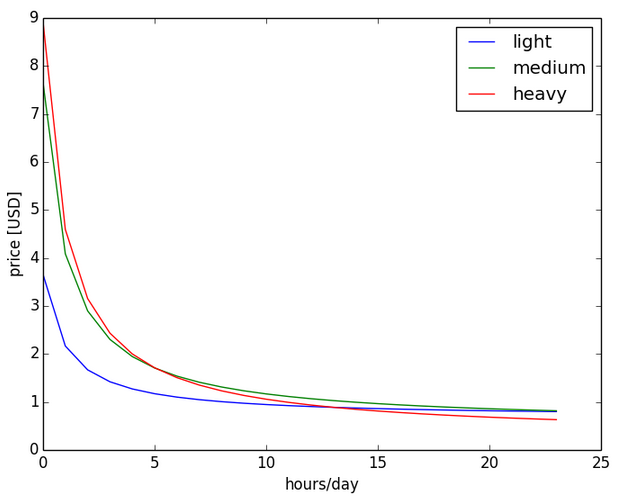
\includegraphics[width=\linewidth]{figures/m2_4xlarge}
  \caption{\textit{cph} results for Amazon AWS m2.4xlarge reserved instance rented for 1 year~\cite{AWS:light}~\cite{AWS:medium}~\cite{AWS:heavy}}
  \label{fig:m2_4xlarge}
\end{figure}

\subsection{Key distance indicator and total cost}

The key distance indicator was calculated based on Algorithm~\ref{alg:distance_from_optimality}. 
Total cost was calculated based on total uptime and pricing scheme assignment. Results are presented in Table~\ref{tab:kdi_and_cost}.

\begin{table}[h]
\begin{center}
    \begin{tabular}{| l | l | l |}
    \hline
    \textbf{Indicator} & \textbf{Scheme 1} & \textbf{Scheme 2} \\
    \hline
    Total cost & \$8 177 048 & \$5 637 418 \\
    \hline
    KDI & +3 215 231 & +5 431 137 \\
    \hline
%    Total CPU & 15972217.38 & 15972217.38 \\
%    \hline
%    Total Memory & 30676363.36 & 30676363.36 \\
%    \hline
%    Number of tasks & 1234716525 & 1234716525 \\
%    \hline
    \end{tabular}
\end{center}
\caption{KDI and total cost for cluster}
\label{tab:kdi_and_cost}
\end{table}

KDI for Scheme 1 and 2 is a positive number, which is expected based on 82\% of heavy scheme assignment and 23.36 hours of uptime per day on average.
Scheme 1 is 31\% more expensive than Scheme 2 and this is expected as well as \textit{cph} values are higher for Scheme 1. 

\section{Recognize inefficiencies using threshold-based report}

KDI can be used to find inefficiencies.  Any value below 0 indicates non-optimal usage for a given scheme. 
A user can specify a threshold to find non-optimal cases. We will assume that non-optimal usage within the cluster is when machine reports negative KDI values for the whole trace period.
 These criteria identified 932 and 937 machines for Scheme 1 and 2 respectively. Detailed results split by cost and resource utilization are presented in Table~\ref{tab:threshold_based_report}.

\begin{table}[h]
\begin{center}
    \begin{tabular}{| l | l | l |}
    \hline
    \textbf{Property} & \textbf{Scheme 1} & \textbf{Scheme 2} \\
    \hline
    Number of machines to tune & 932 & 937 \\
    \hline
    Total cost & \$657 200 & \$532 841 \\
    \hline
    CPU capacity to accommodate & 1 320 781.36 & 1 327 202.18 \\
    \hline
    Memory capacity to accommodate & 4 286 742.06 & 4 303 983.31 \\
    \hline
    Number of tasks to execute & 118869614 & 119367988 \\
    \hline
    Total uptime & 648519 & 651899 \\
    \hline
    Average cost per hour & \$1.0134 & \$0.817 \\
    \hline
    Average cost per task & \$0.00553  & \$0.00446 \\
    \hline
    \end{tabular}
\end{center}
\caption{Results of report run on cluster with criteria of KDI below 0 for 29 days}
\label{tab:threshold_based_report}
\end{table}

The cost of running identified non-optimal machines is around 8\% and 10\% of total cost for Scheme 1 and 2 respectively.  

\section{Squeeze-them-in suggestion strategy}

Based on Algorithm~\ref{alg:squeeze-them-in} we calculated spare capacity for both schemes. Results are presented in Table~\ref{tab:squeeze-them-in-capacity}

\begin{table}[h]
\begin{center}
    \begin{tabular}{| l | l | l |}
    \hline
    \textbf{Property} & \textbf{Scheme 1} & \textbf{Scheme 2} \\
    \hline
    Total spare CPU & 3 697 171.44 & 6 3 694 240.56  \\
    \hline
    Total spare memory & 6 685 407.83 & 6 682 956.59 \\
    \hline
    \end{tabular}
\end{center}
\caption{Results of spare capacity calculation on the cluster}
\label{tab:squeeze-them-in-capacity}
\end{table}

In both cases, there is more spare capacity than results from Table~\ref{tab:threshold_based_report} require. It indicates we can power off all of the non-optimal machines and investigate an impact on workload and pricing indicators. Results of such an experiment are presented in Table~\ref{tab:squeeze-them-in}. 

\begin{table}[h]
\begin{center}
    \begin{tabular}{| l | l | l |}
    \hline
    \textbf{Property} & \textbf{Scheme 1} & \textbf{Scheme 2} \\
    \hline
    New KDI & +3 500 037 & +5 913 933 \\
    \hline
    KDI change & +8.14\% & +8.16\% \\
    \hline
    New total cost & \$7 519 848 & \$5 104 577.24 \\
    \hline
    Total cost change & -8.04\% & -9.45\% \\
    \hline
    New cost per hour & \$0.9334 & \$0.6339 \\
    \hline
    New cost per task & \$0.0633  & \$0.0428 \\
    \hline
    New CPU average per machine & 47.27 & 47.29 \\
    \hline
    CPU average change & +7.4\% & +7.44\% \\
    \hline
    New memory usage average & 90.79 & 90.83 \\
    \hline
    Memory average change & +7.41\% & +7.45\% \\
    \hline
    New task number average & 3654 & 3655 \\
    \hline
    Task average change & +7.4\% & +7.45\% \\
    \hline
    \end{tabular}
\end{center}
\caption{Cluster statistics with non-optimal machines powered off}
\label{tab:squeeze-them-in}
\end{table}

The KDI increased by above 8\% for both schemes. This is expected as we removed machines with negative KDI values. The total cost decreased by 8.04\% and 9.45\% for Scheme 1 and 2 respectively. This is also expected. We noticed a correlation between the increase of KDI and decrease of total cost. However, there is a trade-off in terms of resource utilization, which increased around 7.4\% on average. A user has to decide whether this is acceptable for his specific workload SLAs. It might work well for under-utilized clusters with a low peak-to-mean ratio. For high peak-to-mean workloads, the real difference in utilization patterns can be higher than detected by averages. To measure SLAs in these environments, we would have to use more specific metrics like requests per second or queries per second during peak. 


\section{New capacity configuration suggestion}

We used Algorithm~\ref{alg:new_configuration} to come up with new configuration suggestions based on the uptime of machines from Table~\ref{tab:threshold_based_report} and Scheme 1 and 2 pricing details. \\
The algorithm analyzed all three \textit{intersection points} available for each scheme and returned total cost and number of machines required. Results are presented in Table~\ref{tab:new-cap-scheme1} and~\ref{tab:new-cap-scheme2}.

\begin{table}[h]
\begin{center}
    \begin{tabular}{| l | l | l |}
    \hline
    \textbf{Scheme} & \textbf{Machines} & \textbf{Total cost} \\
    \hline
    Light & 1397 & \$770 417.58 \\
    \hline
    Medium & 1720 & \$876 376.34 \\
    \hline
    Heavy & 972 & \$604 274.61\\
    \hline
    \end{tabular}
\end{center}
\caption{New capacity configuration suggestions for Scheme 1}
\label{tab:new-cap-scheme1}
\end{table}

\begin{table}[h]
\begin{center}
    \begin{tabular}{| l | l | l |}
    \hline
    \textbf{Scheme} & \textbf{Machines} & \textbf{Total cost} \\
    \hline
    Light & 1597 & \$567 273.49 \\
    \hline
    Medium & 3727 & \$998 186.23 \\
    \hline
    Heavy & 972 & \$410 041.68 \\
    \hline
    \end{tabular}
\end{center}
\caption{New capacity configuration suggestions for Scheme 2}
\label{tab:new-cap-scheme2}
\end{table}

An interesting pattern raised - a medium is always the least optimal choice and heavy is the best. The suggestion to run heavy configuration for Scheme 1 would save 8.05\% compared to non-optimal machines set and 0.0065\% from total cost. Scheme 2 would save 23\% compared to non-optimal machines set and 0.022\% from total cost. KDI increased for both schemes. Scheme 1 noted 8.42\% change and Scheme 2 8.31\%. Light and medium suggestions turned out to be more expensive and were excluded from the rest of considerations. \\

As opposed to the previous algorithm, this one does not violate SLAs. The new suggested capacity handles the same amount of uptime using the same resource configuration as the rest of the cluster. 


\section{Validate correlation of total cost and KDI}

We aggregated all of the generated suggestions and graphed values of KDI and total cost changes on Figure~\ref{fig:kdi_to_cost}. 
By design, KDI reports higher positive number when usage is more optimal. We can see that for each suggestion generated by both algorithms, KDI increased and the total cost dropped. This suggests a direct correlation between these values. However, higher KDI increase did not directly decreases the total cost further.  

\begin{figure}[H]
	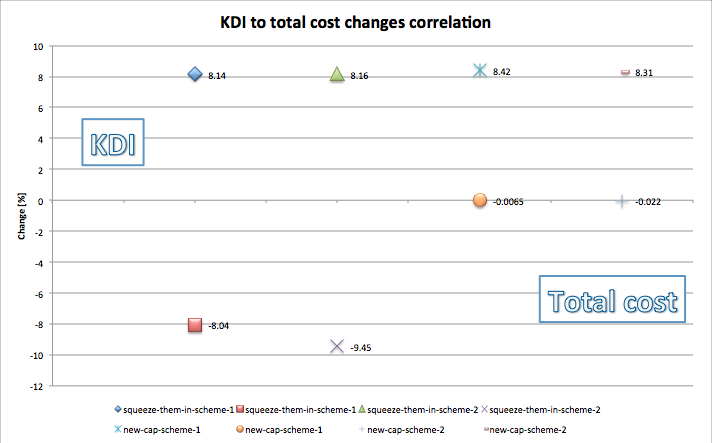
\includegraphics[width=\linewidth]{figures/kdi_to_cost}
	\caption{KDI to total cost correlation}
	\label{fig:kdi_to_cost}
\end{figure}

%%%%%%%%%%%%%%%%%%%%%%
%%% CONCLUSION AND 
%%% FUTURE WORK
%%%%%%%%%%%%%%%%%%%%%%

\chapter{Conclusion and Future Work}

\myparagraph{Conclusion}
We proposed an uptime-based approach for capacity planning in Cloud environments. 

At first, we selected metrics required to make data-driven decisions. We applied transformations and aggregations to extract relevant data on a daily, per machine basis. Based on that, we calculated and applied our proposed key indicators -~\textit{cph, ip(scheme1, scheme2), KDI}- and assessed the state of Google trace data's optimality. It turned out that based purely on~\textit{KDI} values, around 7-8\% of machines could benefit from reconfiguration. We used this data as an input to our two suggestion algorithms. 

Squeeze-them-in algorithm suggested that there is enough spare capacity to power off non-optimal machines. As a result, the total cost dropped by 8.04\% and 9.45\% for both analyzed pricing configurations. Obviously, this came with a trade-off related to a higher utilization of the cluster. CPU and memory averages increased by around 7\%. There is not enough data to state whether this is acceptable or not. We would have to make assumptions, therefore the final evaluation of the algorithm's usefulness is delegated to the user and his specific requirements.

New capacity configuration algorithm suggested alternative VM arrangements. Some of them turned out to be worse and got excluded from further analysis. It is worth to note that suggestions that were actually better, in this context - cheaper, contained only Heavy instances for both analyzed schemes. They yielded improvements in a range from 8 to 23\% compared to the previous non-optimal configuration and from 0.0065 to 0.022\% in relation to the total cost.

It is somewhat safe to assume that when~\textit{KDI} is negative, a configuration is non-optimal. It indicates that there are more machines that report negative~\textit{KDI} values than positive and it is something worth to investigate. However, when cluster-wide~\textit{KDI} equals 0 or is positive, the number itself does not represent a lot of insight. There might be a situation when half of the machines run in a quite optimal way and yield high~\textit{KDI} values and, at the same time, the other half is non-optimal. As a result of that, we cannot tie a positive~\textit{KDI} value to indicate an optimal configuration. A positive value is better than negative, however, even this statement was not formally proved and can yield surprising results. Nevertheless, we discovered a correlation between~\textit{KDI} increase and total cost decrease. It is not a linear correlation - higher~\textit{KDI} increases does not seem to cause bigger cost decreases. This is an exciting discovery that can be validated further in future work using bigger data sets and different environments. 
The fact these two metrics correlate can be used to validate new suggestion algorithms.

\myparagraph{Future Work}

Each aggregation, key indicator and algorithm was designed as a proof of concept and can be developed and evaluated further. However, there are few key contributions that would make this thesis more valuable in real-life scenarios.

\begin{enumerate}
\item Capacity growth trend calculation. Update algorithms to suggest optimal configurations using the trend. 
\item Predict price changes and discounts. Moore's Law still works~\cite{7057609} and optimizations that affect future should take this into account.
\item Calculate a cost of migration to a newly suggested configuration. This cost should be added to a total cost that is calculated.
\item Use horizon charts\footnote{\url{http://vis.berkeley.edu/thesiss/horizon}} to visualize~\textit{KDI} values. It would be an improvement to the threshold-based report as there might be a set of machines just below the threshold that are not recognized by the report.
\item Research whether~\textit{KDI} correlates to a total cost in bigger sets of data and various pricing environments. If this was true, KDI could be used to validate suggestion algorithms results. 

%%
%%Also, just to reiterate a couple of things I mentioned
%%before: while a realistic algorithm would have to
%%account for predicted prices, predicted discounts,
%%etc I think you should initially focus on a scenario
%%where the pricing scheme is fixed (though the prices
%%themselves will vary in time, naturally). And it's very
%%important that you produce 'something' working e.g.
%%an implementation of your algorithm, tied into the
%%data and so on.

%%

\end{enumerate}

%%%%%%%%%%%%%%%%%%%%%%
%%% REFERENCES 
%%%%%%%%%%%%%%%%%%%%%%

\newpage

\label{endpage}
\bibliography{bib}{}
\bibliographystyle{plain}
\end{document}
\end{document}

\end{article}